%%%%%%%%%%%%%%%%%%%%%%%%%%%%%%%%%%%%%%%%%%%%%%%%%%%%%%%%%%%%%%%%%%%%%%%%
\section{Introduction}
\label{sec:intro}
%%%%%%%%%%%%%%%%%%%%%%%%%%%%%%%%%%%%%%%%%%%%%%%%%%%%%%%%%%%%%%%%%%%%%%%%

Object detection has numerous applications, from mobile phones, cameras and IoT devices, to drones and autonomous cars. With the aid of machine learning (ML), object detection incorporates the classification of the object, i.e., the machine can now asses, with certain probability, what is the object which it has detected (Figure \ref{fig:detection_example}). The combination of computer vision (CV) and ML for on-the-fly object detection and classification, is one of the key points
for enabling the progress of autonomous cars research in recent years.

Object detection algorithms work best on graphical processing units (GPUs). GPUs are implemented with a large number of cores (\textit{streaming multiprocessors} (SMs)), therefore the high parallelism enables algorithms, such as object detection and machines learning, to run faster than on a CPU.

With the increasing demand for low-energy modules, NVIDIA has started to manufacture an embedded platform called Jetson. We have received the Jetson TX1 to explore the performance of different object detection algorithms. NVIDIA's Jetson TX1 is an embedded system-on-module (SoM) with quad-core ARM Cortex-A57, 4GB LPDDR4 and integrated 256-core Maxwell GPU. It is useful for deploying computer vision and deep learning in 10 watts of power.

In this paper we will discuss and analyze the performance of two algorithms on a Jetson TX1 platform: (1) \textit{Single Shot MultiBox Detector} (SSD) \cite{liu2016ssd}, as implemented with Caffe, and (2) \textit{You Only Look Once} (YOLO) \cite{redmon2016you}.

The remainder of this paper is organized as follows: Section \ref{sec:results} presents SSD and YOLO performance on Jetson TX1; Section \ref{sec:profiling} analyzes the algorithms execution using NVIDIA Visual Profiler; Section \ref{sec:installation} shares installation and execution tips we have gathered along the way, and we conclude in Section \ref{sec:conclusion}.

\begin{figure}[t]
	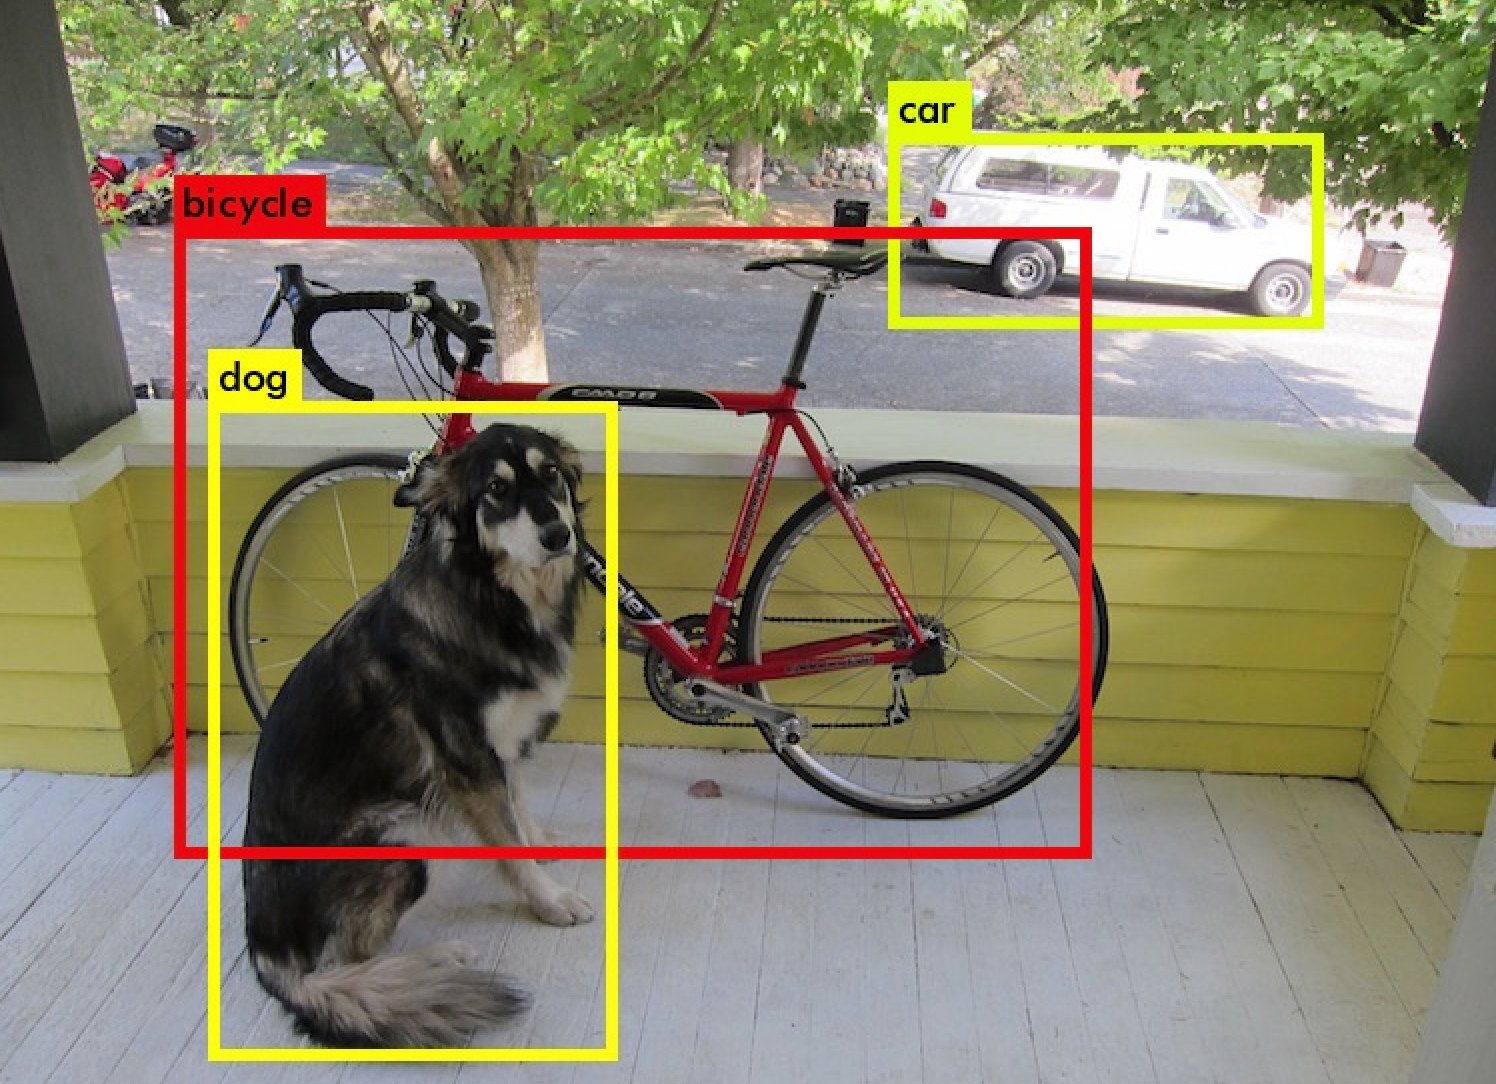
\includegraphics[width=0.48\textwidth]{./imgs/detection_example.png}
	\caption{Object detection example using YOLO}
	\label{fig:detection_example}
\end{figure}
